\documentclass[10pt,twocolumn]{article}

\usepackage[a4paper,top=17mm,bottom=19mm,left=16mm,right=16mm,columnsep=7mm]{geometry}
\usepackage[T1]{fontenc}
\usepackage{newtxtext,newtxmath}
\usepackage{microtype}
\usepackage{graphicx}
\usepackage{booktabs}
\usepackage{array}
\usepackage{amsmath}
\usepackage{siunitx}
\usepackage{xcolor}
\usepackage{caption}
\usepackage{subcaption}
\usepackage{cuted}
\usepackage{tabularx}
\usepackage{tikz}
\usetikzlibrary{arrows.meta,positioning,fit,calc}
\usepackage[numbers,sort&compress]{natbib}
\renewcommand{\bibfont}{\footnotesize}
\setlength{\bibsep}{1.5pt plus 0.5pt}
\usepackage[colorlinks=true,allcolors=blue!55!black]{hyperref}

\definecolor{YouthBlue}{HTML}{1F77B4}
\definecolor{IdentityTeal}{HTML}{2A9D8F}
\definecolor{SOKMRed}{HTML}{C94C4C}
\definecolor{SoftGray}{HTML}{F1F3F5}
\definecolor{TextGray}{HTML}{4D5156}

\graphicspath{{figures/}} % 画像を入れるフォルダを指定
\captionsetup{font=footnotesize,labelfont=bf,justification=justified,singlelinecheck=false}
\setlength{\parindent}{1em}
\setlength{\parskip}{0pt}
\setlength{\textfloatsep}{8pt plus 2pt minus 2pt}
\setlength{\floatsep}{7pt plus 2pt minus 2pt}
\setlength{\intextsep}{7pt plus 2pt minus 2pt}
\setlength{\stripsep}{6pt plus 1pt minus 1pt}
\sisetup{detect-all,round-mode=places,round-precision=4}

% カスタムコマンド
\newcommand{\SOKM}{SOKM}
\newcommand{\RiskScore}{\textit{Risk Score}}

\begin{document}
\raggedbottom

% タイトル部分はご自身の担当セクション名に合わせて調整してください
\twocolumn[
\begin{@twocolumnfalse}
\begin{center}
{\LARGE\bfseries Multi-Dimensional Safety Profiling:\par}
\vspace{2pt}
{\Large\bfseries Pluripotency and Genomic Stress Risks in Partial Reprogramming\par}
\vspace{8pt}
{\large Kei Hasegawa}\par
\vspace{10pt}
\end{center}

\vspace{8pt}
\hrule
\vspace{10pt}
\end{@twocolumnfalse}
]

\section{Methods}

\subsection{Risk Score Definition and Quantification}

\subsubsection{Risk Gene Selection and Refinement}
To accurately quantify the adverse effects associated with partial reprogramming, we iteratively refined our risk gene signatures to ensure biological specificity and construct validity. The progression of our gene lists, corresponding to the files available in our GitHub repository, is summarized in Table~\ref{tab:gene-lists}.

% 遺伝子リスト変遷の表（見開き幅）
\begin{strip}
\noindent\begin{minipage}{\textwidth}
\centering
\captionof{table}{Evolution of Risk Gene Signatures and Corresponding GitHub Files.}
\label{tab:gene-lists}
\small
\begin{tabularx}{\textwidth}{l l X}
\toprule
\textbf{Version} & \textbf{Filename (GitHub)} & \textbf{Description \& Rationale for Revision} \\
\midrule
Version 1 & \texttt{risk\_genes.csv} & Initial mapping of raw MSigDB HALLMARK pathways \citep{liberzon2015} and the SenMayo gene set \citep{saul2022} to three axes: Dedifferentiation, Inflammation, and Tumor. Flaws identified: Dedifferentiation included mesenchymal markers; Tumor contained >800 normal cell proliferation markers. \\
Version 2 & \texttt{risk\_genes\_adjusted.csv} & Renamed ``Tumor'' to ``Genomic Stress'' and restricted to \texttt{DNA\_REPAIR} and \texttt{P53\_PATHWAY} (338 genes) to prevent penalizing physiological cell cycle arrest induced by \SOKM{} stress. \\
Version 3 & \texttt{risk\_genes\_housekeeping\_revised.csv} & Removed genes present in the \texttt{HOUNKPE\_HOUSEKEEPING\_GENES} database \citep{hounkpe2021} to minimize baseline transcriptomic noise. \\
Version 4 (Final) & \texttt{finalized\_risk\_genes\_list.csv} & Addressed trajectory mapping issues (mesenchymal markers falsely lowered the score). Dedifferentiation was restricted strictly to 10 pluripotency markers and renamed ``Pluripotency.'' Inflammation was entirely removed, as partial reprogramming physiologically suppresses aging-associated inflammation \citep{roux2022}. \\
\bottomrule
\end{tabularx}
\end{minipage}
\end{strip}

Initially (Version 1), we mapped raw MSigDB HALLMARK pathways \citep{liberzon2015} and senescence-associated genes from the SenMayo dataset \citep{saul2022} to three proposed axes. However, biological validation revealed critical confounding factors. The original Dedifferentiation axis included mesenchymal markers, which incorrectly penalized normal mesenchymal stem cells (MSCs) for maintaining their somatic identity. Similarly, the Tumor axis contained normal cellular proliferation genes, which falsely flagged the physiological cell cycle arrest induced by \SOKM{} stress as a tumorigenic event.

To resolve these artifacts, Version 2 redefined the tumorigenesis axis as ``Genomic Stress,'' utilizing strictly DNA repair and p53 pathways, and Version 3 filtered out housekeeping genes \citep{hounkpe2021}. Ultimately, the final model (Version 4) was established upon realizing that the initial pseudotime projection was inverted, causing the dedifferentiation score to artificially drop. Consequently, the axis was redefined as ``Pluripotency Risk'' and strictly limited to 10 established pluripotency markers (e.g., \textit{Nanog, Pou5f1, Sox2}). Notably, the ``Inflammation'' axis was entirely removed; previous research demonstrated that partial reprogramming naturally suppresses aging-associated inflammation \citep{roux2022}, meaning this axis inadvertently measured rejuvenation efficacy rather than intervention-induced toxicity.

\subsubsection{Positive Control Datasets}
To validate the construct validity of our finalized axes, we employed independent transcriptomic datasets. For the Pluripotency Risk, we utilized a time-course bulk RNA-seq dataset tracking the cellular transition from MEFs to iPSCs (Velychko et al., 2019 \citep{velychko2019}). For the Genomic Stress Risk, we analyzed bulk transcriptomes from an \textit{in vivo} MSC-to-Kaposi's sarcoma progression model (Naipauer et al., 2019 \citep{naipauer2019}). 

\subsubsection{Scoring Algorithm and Donor-Level Aggregation}
Single-cell risk scores were computed using the \texttt{sc.tl.score\_genes} function in Scanpy (parameters: \texttt{ctrl\_size=50}, \texttt{n\_bins=25}, \texttt{random\_state=42}) on transcriptomes normalized to 10{,}000 counts per cell and log1p-transformed. For trajectory analysis specifically in the Roux et al. dataset \citep{roux2022}, velocity pseudotime was mathematically inverted ($1.0 - \text{pseudotime}$) to align with the intuitive biological progression from somatic baseline (0.0) to pluripotency (1.0). 

To evaluate safety at the biological replicate level, we aggregated single-cell scores into donor-level contracts. We adopted the median rather than the mean as our primary measure of central tendency because the median is substantially more robust against extreme technical outliers common in single-cell transcriptomic data. The primary tail-risk metric, ``High-Risk Cell Fraction,'' was defined as the proportion of \SOKM-treated cells exceeding the 95th percentile risk score of age-matched, untreated control cells (NegCtrl).


\section{Results}

\subsection{Multi-Dimensional Safety Profiling}

\subsubsection{Validation of Risk Modules using Positive Controls}
Before evaluating the \textit{in vivo} \SOKM{} dataset, we validated our finalized Risk Modules against established positive control datasets (Fig.~\ref{fig:positive-controls}). The Pluripotency Risk Score demonstrated robust construct validity, exhibiting a massive and specific spike in fully reprogrammed iPSCs and ESCs. Furthermore, it accurately captured the continuous, incremental increase in pluripotency risk across intermediate states from baseline MEFs to fully dedifferentiated cells (Fig.~\ref{fig:positive-controls}A). 

In contrast, while the Genomic Stress Risk Score successfully identified a general upward trend from normal MSCs to pre-cancerous states and ultimately to \textit{in vivo} sarcomas, it exhibited higher intra-group variance and instability, likely exacerbated by the small sample size of the dataset. Notably, certain cells within the tumor fraction presented scores comparable to the normal baseline, indicating that the Genomic Stress axis possesses slightly lower quantitative resolution and separability compared to the highly targeted Pluripotency axis (Fig.~\ref{fig:positive-controls}B).

\begin{strip}
\noindent\begin{minipage}{\textwidth}
\centering
\begin{minipage}[t]{0.48\textwidth}
\centering
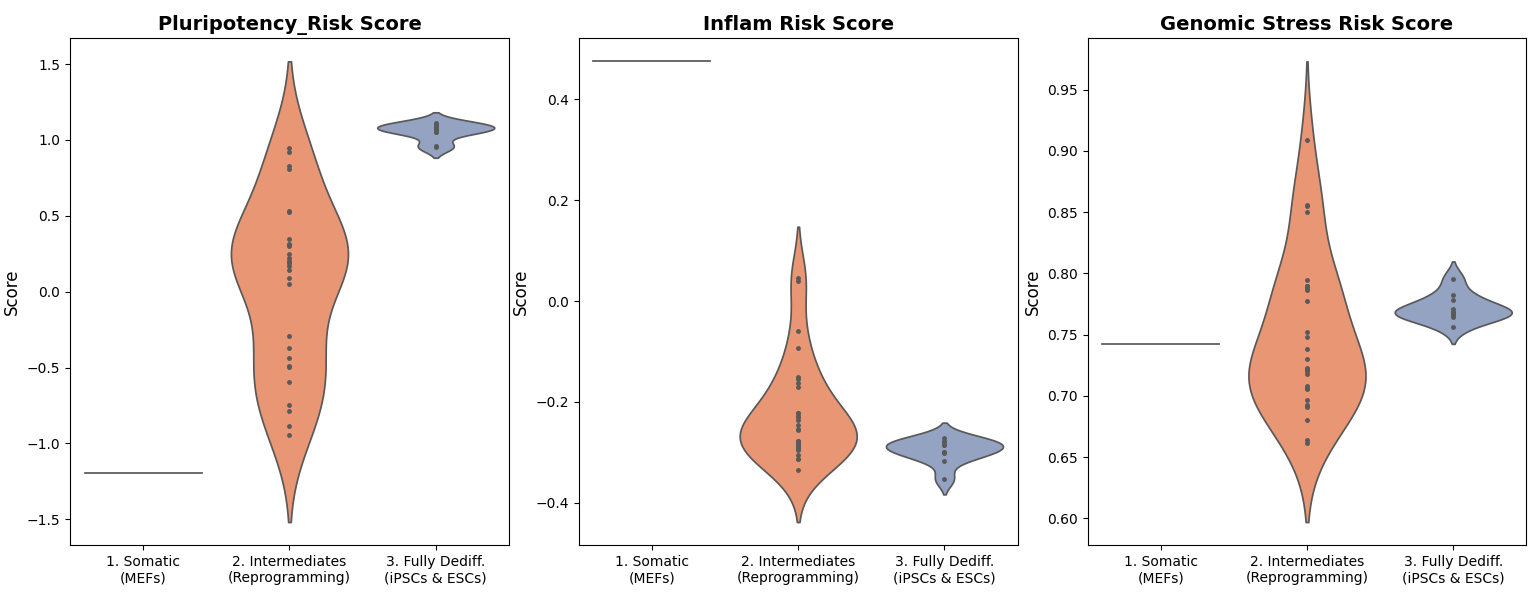
\includegraphics[width=\linewidth]{pluripotency_Positive_Control_Validation.png}
\small\textbf{A.} Pluripotency Risk Validation (Velychko et al.)
\end{minipage}\hfill
\begin{minipage}[t]{0.48\textwidth}
\centering

\includegraphics[width=\linewidth]{Genomic_Stress_positive_control_PDGFRA.png}
\small\textbf{B.} Genomic Stress Risk Validation (Naipauer et al.)
\end{minipage}
\captionof{figure}{Validation of Risk Modules using Positive Controls. (A) The Pluripotency score shows a continuous increase across reprogramming intermediates. (B) The Genomic Stress score demonstrates an upward trend towards sarcomas, albeit with higher variance and instability due to limited sample sizes.}
\label{fig:positive-controls}
\end{minipage}
\end{strip}

\subsubsection{Risk Dynamics along the Reprogramming Trajectory}
We next applied our scoring modules to the Roux et al. \textit{in vivo} MSC dataset \citep{roux2022} to observe risk dynamics along the reprogramming pseudotime (Fig.~\ref{fig:trajectory}). Consistent with our rationale for removing it from the safety module, the Inflammation score steadily decreased as pseudotime advanced, corroborating the premise that partial reprogramming alleviates age-related inflammatory phenotypes. 

\begin{strip}
\noindent\begin{minipage}{\textwidth}
\centering
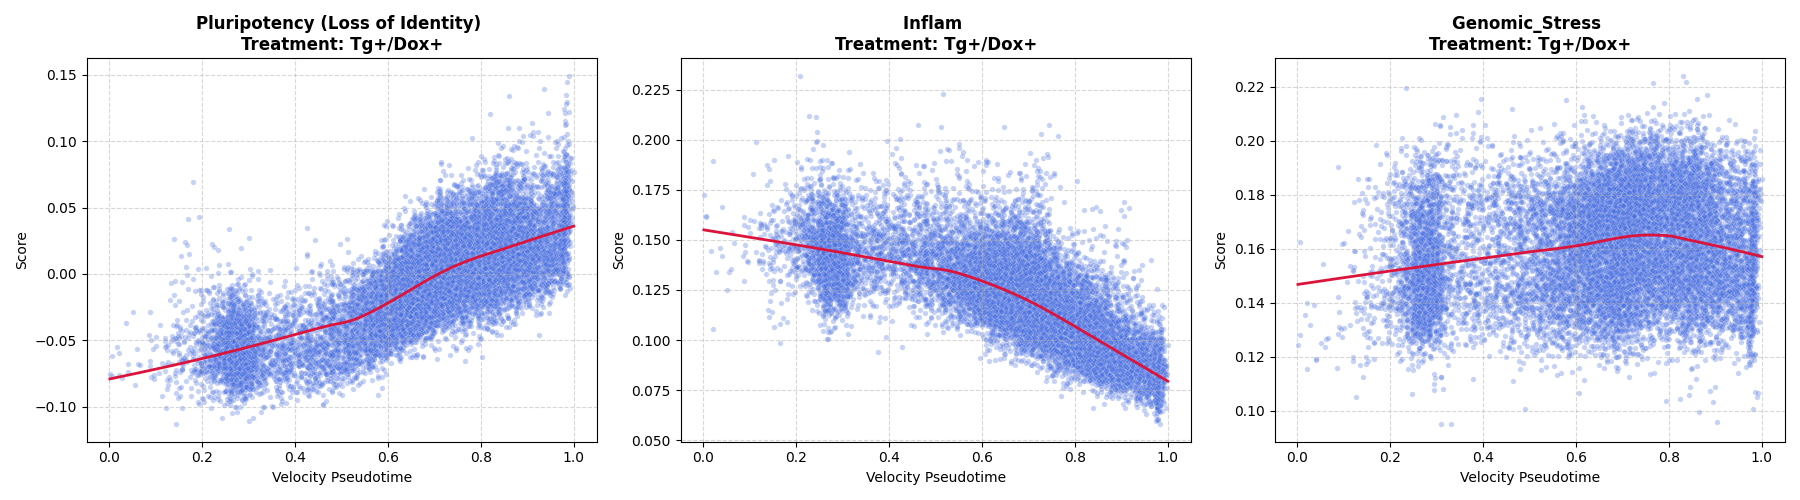
\includegraphics[width=0.9\textwidth]{Finalized_risk_score_roux_with_inflam.png}
\captionof{figure}{Risk Dynamics along the Reprogramming Trajectory. Scatter plots with LOWESS regression lines illustrating the progression of Pluripotency, Genomic Stress, and Inflammation scores across the corrected velocity pseudotime in the \SOKM{} treated arm.}
\label{fig:trajectory}
\end{minipage}
\end{strip}

The Pluripotency Risk Score remained relatively stable during the early phases but spiked sharply at the distal end of the trajectory, confirming that severe loss of somatic identity is a late-stage consequence of continuous \SOKM{} expression. The Genomic Stress Risk Score displayed a gradual elevation up to a pseudotime of approximately 0.8, followed by a slight decline at the trajectory's terminus. We hypothesize that this late-stage drop reflects a survivorship bias: cells that accumulate excessive, unresolvable genomic stress likely undergo apoptosis. Consequently, the cells that successfully reach the final highly dedifferentiated state have either evaded these stress pathways or completely resolved the DNA damage, resulting in a lower measured stress score.

\subsubsection{Donor-Level Safety Profiling: Central Tendency vs. Tail Risk}
To assess safety in a translationally relevant manner, we aggregated the single-cell scores into donor-level metrics (Fig.~\ref{fig:donor-safety}). For Pluripotency Risk, \SOKM{} treatment (Tg+/Dox+) induced a drastic elevation across all metrics---not only in the median score but profoundly in the upper-tail risk (p95) and the high-risk cell fraction. Interestingly, while aged control cells (NegCtrl) exhibited slightly higher baseline pluripotency risk than young controls, the \SOKM-induced pluripotency risk was notably higher in \textit{Young} cells. We postulate that the younger epigenome is inherently more plastic and responsive to Yamanaka factors, enabling these cells to traverse the epigenetic landscape more rapidly and breach the critical pluripotency threshold at higher frequencies.

Regarding Genomic Stress, \SOKM{} treatment elevated the median risk score; however, the gap between treatment and control arms narrowed when examining the upper-tail risks. In most cases, Aged donors exhibited higher genomic stress scores than Young donors. This suggests that rather than generating a distinct, hyper-stressed ``rogue'' subpopulation, \SOKM{} treatment elevates the overall baseline of genomic stress uniformly across the population, with aging inherently dictating the baseline variance and susceptibility.

\begin{strip}
\noindent\begin{minipage}{\textwidth}
\centering
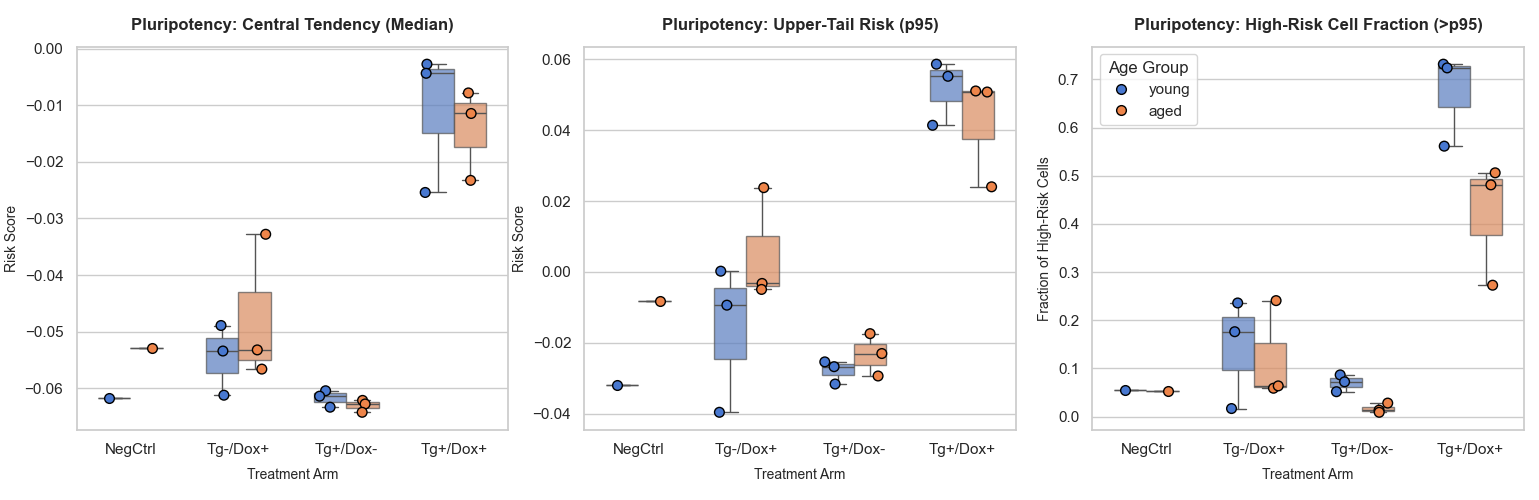
\includegraphics[width=0.9\textwidth]{pluripotency_risk_score_donor_level_plot.png}\\[10pt]
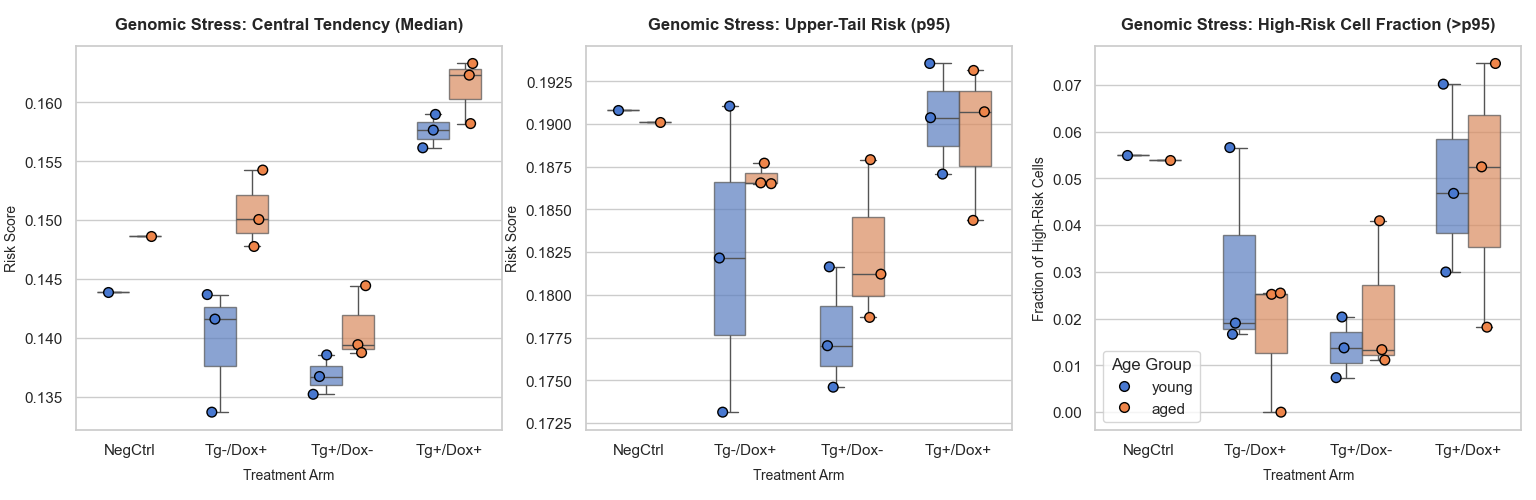
\includegraphics[width=0.9\textwidth]{genomic_stress_risk_score_donor_level_plot.png}
\captionof{figure}{Donor-Level Safety Profiling in GSE176206. Top panels: Pluripotency Risk Score. Bottom panels: Genomic Stress Risk Score. \SOKM{} treatment drastically elevates pluripotency risk, whereas genomic stress exhibits a more uniform baseline shift.}
\label{fig:donor-safety}
\end{minipage}
\end{strip}

\section{Discussion}

\subsection{Risk Score Contributions}

\subsubsection{The Necessity of Multi-layered Profiling}
A primary objective of our safety profiling was to identify whether \SOKM-induced adverse events manifest as uniform population shifts or as rare, highly aberrant ``tail'' events. While our results indicated that genomic stress largely manifests as a population-wide baseline shift, the pluripotency risk exhibited a massive elevation across the entire cellular population, alongside a profound expansion of the high-risk cell fraction. Traditional bulk RNA-seq or single-cell analyses relying exclusively on population means are highly susceptible to masking these heterogeneous cellular responses. Therefore, our multi-layered framework---which calculates single-cell variances and aggregates them into strictly defined donor-level tail-risk metrics---is indispensable for evaluating reprogramming modalities where even a minuscule fraction of dedifferentiated or stressed cells can lead to dysplasia, general abnormal cellular generation, or fatal teratoma formation.

\subsubsection{Methodological Limitations and Future Gene Selection}
We acknowledge several limitations in our current methodology. First, the positive control datasets lacked fine-grained temporal metadata (such as single-cell pseudotime), which limited our ability to strictly align the control validation with the \textit{in vivo} \SOKM{} trajectory. Additionally, while the 10-gene Pluripotency axis demonstrated exceptional specificity, the Genomic Stress axis---derived from hundreds of broadly defined MSigDB HALLMARK genes \citep{liberzon2015}---introduced noticeable noise, hindering clear tumor separation in our positive controls.

Future iterations must move beyond generalized HALLMARK pathways. The ideal approach would involve a comprehensive meta-analysis of multiple independent \textit{in vivo} partial reprogramming datasets to extract a data-driven, highly specific signature of genes that are both exclusively perturbed by \SOKM{} and definitively linked to oncogenesis and aberrant pluripotency acquisition. We refrained from performing this extraction solely on the Roux dataset \citep{roux2022} to strictly avoid model overfitting. Ultimately, the predictive validity of these transcriptomic risk scores must be corroborated using datasets that explicitly track long-term \textit{in vivo} teratoma incidence.

\subsubsection{Bridging Safety Profiling with Generative AI}
The ultimate goal of partial reprogramming is to define a therapeutic ``Safe Zone''---a specific transcriptomic state where rejuvenation is maximized while pluripotency and genomic stress risks remain perfectly suppressed. In our current framework, fully automated identification of this zone is bottlenecked by data formatting discrepancies between generative models (e.g., Geneformer's perturbation embeddings) and conventional transcriptomic score quantification (e.g., Scanpy). Currently, our optimal strategy is iterative: utilizing Generative AI for hypothesis generation regarding safe perturbation targets, followed by rigorous validation using our multidimensional Risk and Youth scoring models. Looking forward, the seamless, end-to-end integration of \textit{in silico} AI generation with single-cell transcriptomic safety profiling will be the definitive key to unlocking safe and scalable cellular rejuvenation therapies.

% 必要に応じてチームの共有.bibファイルを使用してください
% 以下の文献リストはダミーとして直接記述していますが、
% 実際には \bibliography{references} を有効化して管理することを推奨します。
\bibliographystyle{unsrtnat}
\bibliography{references}


\end{document}